\documentclass[aspectratio=169, table]{beamer}
\usepackage[utf8]{inputenc}
\usepackage[T1]{fontenc}
\usepackage{graphicx}
\usepackage{fontspec} 
\usepackage{xcolor}
\usepackage{tcolorbox}

\setsansfont[
ItalicFont=fonts/TitilliumWeb-Italic.ttf,
BoldFont=fonts/TitilliumWeb-Bold.ttf,
BoldItalicFont=fonts/TitilliumWeb-BoldItalic.ttf,
]{TitilliumWeb-Regular.ttf}

\subtitle{IF120203-Programming Fundamentals}
\title{\Huge {\textbf{01: \\Introduction}}}
\date[Serial]{\scriptsize {PRU/SPMI/FR-BM-18/0222}}
\author[Pradita]{\small {\textbf{PRADITA UNIVERSITY}}}

\usetheme{Pradita} %To change Styles of the ppt

\begin{document}
	
	\begin{frame}
		\titlepage
	\end{frame}
	
	\begin{frame}{Goals}
		\vskip-1cm
		\begin{itemize}
			\item To learn about computers and programming
			\item To compile and run your first Java program
			\item To recognize compile-time and run-time errors
			\item To describe an algorithm with pseudocode
		\end{itemize}
	\end{frame}

	\begin{frame}{The Java Programming Language}
		\vskip-0.5cm
		\begin{itemize}
			\item Safe
			\item Portable
			\item Platform-independent
			\begin{itemize}
				{\small \item Distributed as instructions for a virtual machine}
			\end{itemize}
			\item Vast set of library packages
			\item Designed for the internet
		\end{itemize}
	\end{frame}

	\begin{frame}{Java Versions}
		\vskip1cm
		\rowcolors{2}{blueColor!10}{blueColor!10}
		\begin{tabular}{|c|c|m{10cm}|}
				\hline
				\rowcolor{gray!30}\textbf{\textcolor{blueColor}{Version}} & \textbf{\textcolor{blueColor}{Year}} & \textbf{\textcolor{blueColor}{Important New Features}}	\\ \hline
				1.0 	& 1996	&  	\\ \hline
				1.1		& 1997	& Inner Classes	\\ \hline
				1.2		& 1998	& Swing, Collections framework \\ \hline
				1.3		& 2000	& Performance enhancements		\\ \hline
				1.4		& 2002	& Assertions, XML Support		\\ \hline
				5		& 2004	& Generic classes, enhanced for loop, auto-boxing, enumerations, annotations	\\ \hline
				6		& 2006	& Library improvements			\\ \hline
				7		& 2011	& Small language changes and library improvements	\\	\hline
		\end{tabular}
	\end{frame}

	\begin{frame}{Columns Test}
		\begin{tcolorbox}[standard jigsaw, opacityback=0, opacityframe=0, sharp corners, boxrule=0pt]
			\begin{columns}[T] %T for Top, C for Center, B for Bottom
				\begin{column}{0.5\textwidth}
					Lorem ipsum dolor sit amet, consectetur adipiscing elit, sed do eiusmod tempor incididunt ut labore et dolore magna aliqua. Felis donec et odio pellentesque diam. Facilisis leo vel fringilla est ullamcorper eget nulla facilisi.
				\end{column}
				\begin{column}{0.5\textwidth}
					Lorem ipsum dolor sit amet, consectetur adipiscing elit, sed do eiusmod tempor incididunt ut labore et dolore magna aliqua. Felis donec et odio pellentesque diam. Facilisis leo vel fringilla est ullamcorper eget nulla facilisi. Vulputate ut pharetra sit amet aliquam id diam maecenas.
				\end{column}
			\end{columns}
		\end{tcolorbox}
	\end{frame}

	\section{Section}
	\begin{frame} 
		\frametitle{Tester} 
		%\framesubtitle{The proof uses \textit{reductio ad absurdum}.} 
		\begin{theorem}
			There is no largest prime number. \end{theorem} 
		\begin{enumerate} 
			\item<1-| alert@1> Suppose $p$ were the largest prime number. 
			\item<2-> Let $q$ be the product of the first $p$ numbers. 
			\item<3-> Then $q+1$ is not divisible by any of them. 
			\item<1-> But $q + 1$ is greater than $1$, thus divisible by some prime
			number not in the first $p$ numbers.
		\end{enumerate}
	\end{frame}


\begin{frame2}
	\frametitle{References}
	\begin{tcolorbox}[standard jigsaw, opacityback=0, opacityframe=0, sharp corners, boxrule=0pt]
		\begin{columns}[T] %T for Top, C for Center, B for Bottom
			\begin{column}{0.7\textwidth}
				Jain, H. (2017). Problem Solving in Data Structures \& Algorithms Using C++: Programming Interview Guide.
				
			\end{column}
			\begin{column}{0.3\textwidth}
				
			\end{column}
		\end{columns}
	\end{tcolorbox}
\end{frame2}

\begin{frame3}
	\vskip1cm
	\begin{tcolorbox}[standard jigsaw, opacityback=0, opacityframe=0, sharp corners, boxrule=0pt]
		\begin{columns}[T] %T for Top, C for Center, B for Bottom
			\begin{column}{0.5\textwidth}
				\textbf{\textcolor{white}{Then the tree call process dr each element designated in the tree chart mentioned above. By the way, first flip the position of the tree dr down to the top. 
					Then fill it with its elements according to the tree chart. Take a look at this tree call chart:}}
			\end{column}
			\begin{column}{0.5\textwidth}
				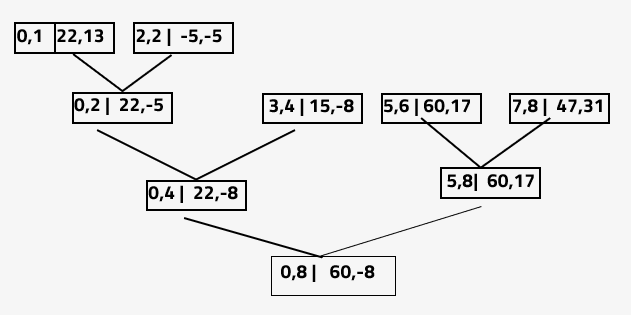
\includegraphics[width=1.2\textwidth]{classFiles/chart.png}
			\end{column}
		\end{columns}
	\end{tcolorbox}
\end{frame3}
	
\begin{frame4}
	\frametitle{Thank You}
\end{frame4}
	
\end{document}